% Options for packages loaded elsewhere
\PassOptionsToPackage{unicode}{hyperref}
\PassOptionsToPackage{hyphens}{url}
%
\documentclass[
]{book}
\usepackage{amsmath,amssymb}
\usepackage{iftex}
\ifPDFTeX
  \usepackage[T1]{fontenc}
  \usepackage[utf8]{inputenc}
  \usepackage{textcomp} % provide euro and other symbols
\else % if luatex or xetex
  \usepackage{unicode-math} % this also loads fontspec
  \defaultfontfeatures{Scale=MatchLowercase}
  \defaultfontfeatures[\rmfamily]{Ligatures=TeX,Scale=1}
\fi
\usepackage{lmodern}
\ifPDFTeX\else
  % xetex/luatex font selection
\fi
% Use upquote if available, for straight quotes in verbatim environments
\IfFileExists{upquote.sty}{\usepackage{upquote}}{}
\IfFileExists{microtype.sty}{% use microtype if available
  \usepackage[]{microtype}
  \UseMicrotypeSet[protrusion]{basicmath} % disable protrusion for tt fonts
}{}
\makeatletter
\@ifundefined{KOMAClassName}{% if non-KOMA class
  \IfFileExists{parskip.sty}{%
    \usepackage{parskip}
  }{% else
    \setlength{\parindent}{0pt}
    \setlength{\parskip}{6pt plus 2pt minus 1pt}}
}{% if KOMA class
  \KOMAoptions{parskip=half}}
\makeatother
\usepackage{xcolor}
\usepackage{longtable,booktabs,array}
\usepackage{calc} % for calculating minipage widths
% Correct order of tables after \paragraph or \subparagraph
\usepackage{etoolbox}
\makeatletter
\patchcmd\longtable{\par}{\if@noskipsec\mbox{}\fi\par}{}{}
\makeatother
% Allow footnotes in longtable head/foot
\IfFileExists{footnotehyper.sty}{\usepackage{footnotehyper}}{\usepackage{footnote}}
\makesavenoteenv{longtable}
\usepackage{graphicx}
\makeatletter
\def\maxwidth{\ifdim\Gin@nat@width>\linewidth\linewidth\else\Gin@nat@width\fi}
\def\maxheight{\ifdim\Gin@nat@height>\textheight\textheight\else\Gin@nat@height\fi}
\makeatother
% Scale images if necessary, so that they will not overflow the page
% margins by default, and it is still possible to overwrite the defaults
% using explicit options in \includegraphics[width, height, ...]{}
\setkeys{Gin}{width=\maxwidth,height=\maxheight,keepaspectratio}
% Set default figure placement to htbp
\makeatletter
\def\fps@figure{htbp}
\makeatother
\setlength{\emergencystretch}{3em} % prevent overfull lines
\providecommand{\tightlist}{%
  \setlength{\itemsep}{0pt}\setlength{\parskip}{0pt}}
\setcounter{secnumdepth}{5}
\usepackage{booktabs}
\usepackage{amsthm}
\makeatletter
\def\thm@space@setup{%
  \thm@preskip=8pt plus 2pt minus 4pt
  \thm@postskip=\thm@preskip
}
\makeatother
\ifLuaTeX
  \usepackage{selnolig}  % disable illegal ligatures
\fi
\usepackage[]{natbib}
\bibliographystyle{apalike}
\IfFileExists{bookmark.sty}{\usepackage{bookmark}}{\usepackage{hyperref}}
\IfFileExists{xurl.sty}{\usepackage{xurl}}{} % add URL line breaks if available
\urlstyle{same}
\hypersetup{
  pdftitle={Machine Learning Guidelines for Natural Resource Management Practitioners},
  pdfauthor={Shih-Ni Prim and Natalie Nelson},
  hidelinks,
  pdfcreator={LaTeX via pandoc}}

\title{Machine Learning Guidelines for Natural Resource Management Practitioners}
\author{Shih-Ni Prim and Natalie Nelson}
\date{2024-02-10}

\begin{document}
\maketitle

{
\setcounter{tocdepth}{1}
\tableofcontents
}
\hypertarget{motivation}{%
\chapter{Motivation}\label{motivation}}

As machine learning (ML) has become a powerful tool, it is noted by some that ML has not been widely used in environmental studies. This booklet is meant to provide a concise guide for natural resource management practitioners. This book serves as a staring point rather than a comprehensive resource, so that practitioners can have a basic understanding of how ML works and how to utilize it to analyze data and answer research questions. When appropriate, we provide case studies and R code as well as other online resources to help the readers on the journey of gaining one powerful tool that seems to be omnipresent in the research world.

\hypertarget{intro}{%
\chapter{Introduction}\label{intro}}

What is machine learning? Essentially, machine learning teaches computer models to look for patterns or make predictions. This might sound like magic or it might seem complicated, but you can think of machine learning models as finding underlying formulas that the data come from. To solve for such formula, many, many mathematical calculations are involved. As we human beings are prone to mistakes, as long as we can identify a framework, we can give the framework and data to a computer model. It is best at repeating meticulous calculations to find a best guess based on our believes of the system and the data we observed.

\hypertarget{supervised-learning}{%
\section{Supervised Learning}\label{supervised-learning}}

\hypertarget{unsupervised-learning}{%
\section{Unsupervised Learning}\label{unsupervised-learning}}

\hypertarget{data}{%
\chapter{Data}\label{data}}

\hypertarget{what-to-do-with-data}{%
\section{What to do with data?}\label{what-to-do-with-data}}

One could argue that data is the single most important ingredient when it comes to machine learning models or any type of analysis. As one might say, junk in, junk out.

\hypertarget{data-requirement}{%
\section{Data Requirement}\label{data-requirement}}

\hypertarget{evaluation}{%
\chapter{Evaluation}\label{evaluation}}

\hypertarget{training-vs-testing}{%
\section{Training vs Testing}\label{training-vs-testing}}

We should first address the concepts of training and testing.

\hypertarget{metrics}{%
\section{Metrics}\label{metrics}}

\hypertarget{continuous-responses}{%
\subsection{Continuous Responses}\label{continuous-responses}}

\hypertarget{discrete-responses}{%
\subsection{Discrete Responses}\label{discrete-responses}}

\hypertarget{cross-validation}{%
\section{Cross Validation}\label{cross-validation}}

One very standard way of evaluation is \(k\)-fold cross validation, commonly with \(k=5\) or \(k=10\). The idea is simple. Divide the data into \(k\) groups. Each time, choose \(k-1\) groups for training, fit the model on the last group, which is the test data, and calculate the desired metrics, such as MSE.

In this way, although less data is used for training, the metrics are more accurate, because now we are not using the same data points for training and testing. Using metrics from cross validation for model selection can ensure that your model does not overfit, which means the model does well with training data but does not generalize well on new data.

\begin{figure}
\centering
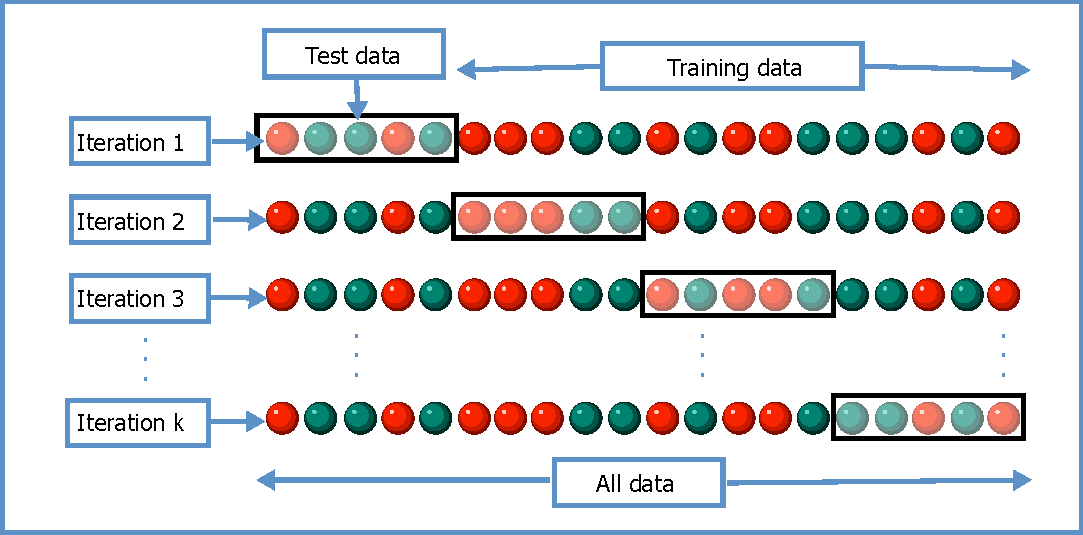
\includegraphics{images/K-fold_cross_validation_EN.pdf}
\caption{\label{fig:unnamed-chunk-4}Image Source: \url{https://en.wikipedia.org/wiki/Cross-validation_(statistics)}}
\end{figure}

\hypertarget{machine-learning-methods}{%
\chapter{Machine Learning Methods}\label{machine-learning-methods}}

Here we provide a list of commonly used machine learning methods and some brief discussion.

\hypertarget{random-forest}{%
\section{Random Forest}\label{random-forest}}

\hypertarget{presentation}{%
\chapter{Presentation}\label{presentation}}

It is also important to present the results in a way that aids rather than impede communication.

\hypertarget{table}{%
\section{Table}\label{table}}

\hypertarget{figure}{%
\section{Figure}\label{figure}}

\hypertarget{ethical-considerations}{%
\chapter{Ethical Considerations}\label{ethical-considerations}}

\hypertarget{reproducibility}{%
\section{Reproducibility}\label{reproducibility}}

To allow for others to reproduce your work, it is important to provide enough details in terms of methods, data processing, code implementation, etc. It is also encouraged to have all the code and data available online in a repository. If parts or all of the data should not be shared publicly, it helps to provide a simulated data set.

\hypertarget{appendix}{%
\chapter{Appendix}\label{appendix}}

\hypertarget{dos-and-donts}{%
\section{Do's and Don'ts}\label{dos-and-donts}}

  \bibliography{book.bib,packages.bib}

\end{document}
